\documentclass{article}

\usepackage{mathtools}
\usepackage{bm}
\usepackage[margin=1.0in]{geometry}
\usepackage{courier}
\usepackage{color}
\usepackage{listings}

\definecolor{dkgreen}{rgb}{0,0.6,0}
\definecolor{gray}{rgb}{0.5,0.5,0.5}

\title{Optimization Methods, Midterm Exam}
\date{2015/10/28}
\author{Matthew Grasinger}

\begin{document}
	
\lstset{language=Matlab,
	keywords={break,case,catch,continue,else,elseif,end,for,function,
		global,if,otherwise,persistent,return,switch,try,while},
	basicstyle=\ttfamily,
	keywordstyle=\color{blue},
	commentstyle=\color{gray},
	stringstyle=\color{dkgreen},
	numbers=left,
	numberstyle=\tiny\color{red},
	stepnumber=1,
	numbersep=10pt,
	backgroundcolor=\color{white},
	tabsize=4,
	showspaces=false,
	showstringspaces=false}
	
\pagenumbering{gobble}
\maketitle
\newpage
\tableofcontents
\newpage
\pagenumbering{arabic}

\section{Problem 1: The Smallest Triangle} \label{sec:small_triangle}

\subsection{Objective}

The objective of the problem is to find the smallest equilateral triangle such that: 
\begin{enumerate}
	\item \label{enum:enclose} The triangle encloses a given set of \textit{n} points in two dimensions, $(x_1, x_2)$.
	\item \label{enum:base_parallel} The base of the triangle is fixed to be parallel to the $x_1$-axis.
	\item \label{enum:base_below} The base of the triangle is below the points.
\end{enumerate}

\subsection{Preliminary Formulation}

We can find a solution to the smallest triangle problem by formulating it as a linear program (LP).
This consists of describing the problem by constraints as a linear system of equations and a cost function that is linear in the unknowns.

\subsubsection{Constraints}

A triangle consists of three lines where each pair of lines meets at a vertex.
For the lines of an equilateral triangle where the base is parallel to the $x_1$-axis, the lines can be given by the three equations,

\begin{eqnarray} \label{eq:d1}
x_2 &=& d_1 \\
\label{eq:d2}
\frac{\sqrt{3}}{2} x_1 + \frac{1}{2} x_2 &=& d_2\\
\label{eq:d3}
-\frac{\sqrt{3}}{2} x_1 + \frac{1}{2} x_2 &=& d_3
\end{eqnarray}

\noindent where $d_1$, $d_2$, and $d_3$ are the three unknowns that construct the triangle.
Alternatively, (\ref{eq:d1}--\ref{eq:d3}) can be written as:

\begin{equation} \label{eq:triangle_lines_la}
\mathbf{a}_i^T \mathbf{x} = d_i
\end{equation}

\noindent where $\mathbf{a}_1 = \begin{bmatrix}0 && 1\end{bmatrix}^T$, $\mathbf{a}_2 = \begin{bmatrix}\frac{\sqrt{3}}{2} && \frac{1}{2}\end{bmatrix}^T$, $\mathbf{a}_3 = \begin{bmatrix}-\frac{\sqrt{3}}{2} && \frac{1}{2}\end{bmatrix}^T$ and $\mathbf{x} = \begin{bmatrix}x_1 && x_2\end{bmatrix}^T$.

Now that we have equations that construct a unique triangle, it is necessary to introduce constraints on $d_1$, $d_2$, and $d_3$.
In plain English, we need ensure that the triangle is constructed such that all of the points lie inside of it.
To express this formally, we need to establish relationships between each point and each line.
Consider the line constructed from $\mathbf{a}_1^T \mathbf{x} = d_1$. When $\mathbf{a}_1^T \mathbf{x} < d_1$, the point $\mathbf{x}$ falls below the line.
We can see then that to satisfy part \ref{enum:base_below} of the problem objective, $d_1$ must not be greater than $\mathbf{a}_1^T \mathbf{x}$ for any point $\mathbf{x}$.
Using similar reasoning we derive the constraints for $d_2$ and $d_3$. The three constraints are formally,

\begin{eqnarray}
\label{eq:const_1} \mathbf{a}_1^T \mathbf{x} &\ge& d_1\\
\label{eq:const_2} \mathbf{a}_2^T \mathbf{x} &\le& d_2 \hspace{0.5in} \forall{\mathbf{x}} \in \left\{ \mathbf{x}_i \right\}_{i=1}^n\\
\label{eq:const_3} \mathbf{a}_3^T \mathbf{x} &\le& d_3
\end{eqnarray}

\noindent where $\left\{ \mathbf{x}_i \right\}_{i=1}^n$ is the sequence of \textit{n} points.

\subsubsection{Cost Function}

Part of the objective of problem \ref{sec:small_triangle} is that the triangle be the smallest triangle possible.
We must therefor derive the size of the triangle as a function of the unknowns.
We can assume that by ``smallest'', what is meant is the triangle be of the least possible area.
The area of an equilateral triangle can be determined from the length of its sides, $Area = \frac{\sqrt{3}}{4} s^2$.
It is sufficient then to derive the length of the triangle's sides as a function of the unknowns.
The length of a line can be determined using the coordinates of the points which the line connects: $\sqrt{(x_{21} - x_{11})^2 + (x_{22} - x_{12})^2}$ where $x_{ij}$ is the $j^{th}$ coordinate of the $i^{th}$ point.
The length of the base of the triangle can be determined by finding where the base intersects each of the other two lines.
We can find the points of intersection by setting equation (\ref{eq:d1}) equal to equation (\ref{eq:d2}) and equation (\ref{eq:d1}) equal to equation (\ref{eq:d3}).
If we set (\ref{eq:d1}) equal to (\ref{eq:d2}) we end up with the following relationship:

\begin{align}
d_1 - x_2 &= d_2 - \frac{\sqrt{3}}{2} x_1 - \frac{1}{2} x_2\\
d_1 &= 2d_2 - \sqrt{3} x_1\\
\label{eq:intersect_1}
x_1 &= \frac{\sqrt{3}}{3}(d_1 - 2d_2) 
\end{align}

\noindent which tells us the $x_1$ coordinate where the two lines intersect.
Similarly, using (\ref{eq:d1}) and (\ref{eq:d3}), the $x_1$ coordinate where the base and Line \ref{eq:d3} insect is,

\begin{equation} \label{eq:intersect_2}
x_1 = \frac{\sqrt{3}}{3}(2d_3 - d_1) 
\end{equation}

\noindent The length of the base is the difference of the two $x_1$-coordinates given by Equations \ref{eq:intersect_1} and \ref{eq:intersect_2}.

\begin{equation} \label{eq:side}
s = \frac{2 \sqrt{3}}{3}(-d_1 + d_2 + d_3)
\end{equation}

\noindent Plugging (\ref{eq:side}) into the equation for the area of the equilateral triangle yields,

\begin{equation} \label{eq:prelim_cost}
Area = \frac{\sqrt{3}}{3}(-d_1 + d_2 + d_3)^2
\end{equation}

\noindent which is the area of the triangle and the cost function for the problem.

\subsection{Standard Form}

The next step in the solution process is to take our preliminary formulation and write it in standard form.
This means writing the cost function as a function that is linear in the unknowns. For the constraints, this means rewriting them in the form $\mathbf{A} \mathbf{x} = \mathbf{b}$.

The cost function in our preliminary formulation is non-linear.
We can simplify this however by recognizing that the solution to minimizing $|-d_1 + d_2 + d_3|$ will also minimize (\ref{eq:prelim_cost}).
Another simplification can be made that is more subtle.
Minimizing $|-d_1 + d_2 + d_3|$ requires minimizing both $(-d_1 + d_2 + d_3)$ and $-(-d_1 + d_2 + d_3)$, but standard form requires that we minimize only one cost function.
If we return to the original objective, part \ref{enum:base_below} tells us that the base of the triangle is below the points.
It is clear that if the base is below the points, and the triangle encloses the points, that lines (\ref{eq:d2}) and (\ref{eq:d3}) must intersect above the base of the triangle (i.e. $x_2$ of their intersection must be greater than $d_1$).
Some elementary algebra shows that this can only occur if $-d_1 + d_2 + d_3 > 0$.
This allows us to simplify the cost function to, $-d_1 + d_2 + d_3$, which satisfies standard form.
The last modification that must be made to the cost function is to rewrite the unknowns as free variables, i.e. as a difference of two non-negative variables, because they should not be bounded from below by zero.
Each $d_i$ then should be rewritten as $u_i - v_i$ where $u_i, v_i$ are non-negative for every index \textit{i}.
More formally,

\begin{equation} \label{eq:lp_cost}
\mathbf{c}^T \mathbf{d}
\end{equation}

\noindent is the cost function we will aim to minimize, where \[\mathbf{c}^T = \begin{bmatrix}-1 & 1 & 1 & -1 & 1 & -1\end{bmatrix}\] and \[\mathbf{d}^T = \begin{bmatrix}u_1 & v_1 & u_2 & v_2 & u_3 & v_3\end{bmatrix}\].

To write the constraints in standard form, we must first write the inequalities as equalities using slack variables.
Equations (\ref{eq:const_1}--\ref{eq:const_3}) with slack variables are

\begin{eqnarray}
\label{eq:lp_const_1} \mathbf{a}_1^T \mathbf{x} &=& d_1 + r_i\\
\label{eq:lp_const_2} \mathbf{a}_2^T \mathbf{x} &=& d_2 - s_i \hspace{0.5in} \forall{\mathbf{x}} \in \left\{ \mathbf{x}_i \right\}_{i=1}^n\\
\label{eq:lp_const_3} \mathbf{a}_3^T \mathbf{x} &=& d_3 - t_i
\end{eqnarray}

\noindent where $r_i$, $s_i$, and $t_i$ are the $3n$ slack variables and are non-negative for all $i = 1, 2, ..., n$.

The slack variables are now part of the unknowns of the problem.
It is therefor necessary to extend our vector of unknowns from the definition given previously to include the slack variables.
Let $\mathbf{u}$ denote all of the unknowns of the problem,

\begin{equation} \label{eq:u}
u = \begin{bmatrix}
u_1 \\ v_1 \\ u_2 \\ v_2 \\ u_3 \\ v_3 \\
r_1 \\ s_1 \\ t_1 \\ %r_2 \\ s_2 \\ t_2 \\
\vdots \\ r_n \\ s_n \\ t_n
\end{bmatrix}
\end{equation}

\noindent so that $\mathbf{u}$ is a vector with $3n + 6$ elements.

The constraints may now be written in the form $\mathbf{A} \mathbf{u} = \mathbf{b}$ where

\begin{equation}
\mathbf{A} = \left[ \begin{smallmatrix}
1 & -1 & 0 & 0 & 0 & 0 & 1 & 0 & 0 & \cdots & 0 & 0 & 0\\
0 & 0 & 1 & -1 & 0 & 0 & 0 & -1 & 0 & \cdots & 0 & 0 & 0\\
0 & 0 & 0 & 0 & 1 & -1 & 0 & 0 & -1 & \cdots & 0 & 0 & 0\\
\vdots & & & & & & \vdots & & & \cdots & & & \vdots\\
1 & -1 & 0 & 0 & 0 & 0 & 0 & 0 & 0 & \cdots & 1 & 0 & 0\\
0 & 0 & 1 & -1 & 0 & 0 & 0 & 0 & 0 & \cdots & 0 & -1 & 0\\
0 & 0 & 0 & 0 & 1 & -1 & 0 & 0 & 0 & \cdots & 0 & 0 & -1\\
\end{smallmatrix} \right]
\end{equation}

\noindent is $3n$ by $3n+6$ matrix, and,

\begin{equation}
\mathbf{b} = \begin{bmatrix}
\mathbf{a}^T_1 \mathbf{x}_1\\
\mathbf{a}^T_2 \mathbf{x}_1\\
\mathbf{a}^T_3 \mathbf{x}_1\\
\vdots\\
\mathbf{a}^T_1 \mathbf{x}_n\\
\mathbf{a}^T_2 \mathbf{x}_n\\
\mathbf{a}^T_3 \mathbf{x}_n
\end{bmatrix}
\end{equation}

\noindent is a vector of $3n$ elements.

We can now write the smallest triangle problem as a linear program in standard form. It is given by,

\begin{eqnarray*}
\min_\mathbf{u} \mathbf{c}^T \mathbf{u}\\
\mathbf{A} \mathbf{u} = \mathbf{b}\\
\mathbf{u} \ge \mathbf{0}
\end{eqnarray*}

\noindent where $\mathbf{c}^T = \begin{bmatrix}-1 & 1 & 1 & -1 & 1 & -1 & 0 & \cdots & 0\end{bmatrix}$ is a vector of $3n + 6$ elements.

\subsection{Problem 1b: Duality}

Investigating the dual of the smallest triangle linear program will be simpler if we reformulate the constraints to use the original inequalities instead of the equalities with slack variables.
The reformulation is,

\begin{equation*}
\mathbf{A} = \begin{bmatrix}
-1 & 1 & 0 & 0 & 0 & 0\\
0 & 0 & 1 & -1 & 0 & 0\\
0 & 0 & 0 & 0 & 1 & -1\\
\vdots & & & & & \vdots\\
-1 & 1 & 0 & 0 & 0 & 0\\
0 & 0 & 1 & -1 & 0 & 0\\
0 & 0 & 0 & 0 & 1 & -1\\
\end{bmatrix}
\end{equation*}

\noindent is $3n$ by $6$ matrix, and,

\begin{equation*}
\mathbf{b} = \begin{bmatrix}
-\mathbf{a}^T_1 \mathbf{x}_1\\
\mathbf{a}^T_2 \mathbf{x}_1\\
\mathbf{a}^T_3 \mathbf{x}_1\\
\vdots\\
-\mathbf{a}^T_1 \mathbf{x}_n\\
\mathbf{a}^T_2 \mathbf{x}_n\\
\mathbf{a}^T_3 \mathbf{x}_n
\end{bmatrix}
\end{equation*}

\noindent is a vector of $3n$ elements.

We can now write the smallest triangle problem as a linear program in a form that is more natural for taking the dual of,

\begin{eqnarray*}
	\min_\mathbf{u} \mathbf{c}^T \mathbf{u}\\
	\mathbf{A} \mathbf{u} \ge \mathbf{b}\\
	\mathbf{u} \ge \mathbf{0}
\end{eqnarray*}

\noindent where \[\mathbf{c}^T = \begin{bmatrix}-1 & 1 & 1 & -1 & 1 & -1\end{bmatrix}\] and \[\mathbf{u}^T = \begin{bmatrix}u_1 & v_1 & u_2 & v_2 & u_3 & v_3\end{bmatrix}\].

\noindent A linear program in this form has a dual of the form:

\begin{eqnarray*}
	\max_{\boldsymbol{\lambda}} \boldsymbol{\lambda}^T \mathbf{b}\\
	\boldsymbol{\lambda}^T \mathbf{A} \le \mathbf{c}^T\\
	\boldsymbol{\lambda} \ge \mathbf{0}
\end{eqnarray*}

\noindent where $\boldsymbol{\lambda}$ is a vector of unknowns with $3n$ elements.
The solution of the dual of this problem would tell us the following:

\begin{itemize}
	\item The cost of the dual is a lower bound on the cost of the primal, and if an optimal solution exists for the dual, not only does this imply that there is an optimal solution for the primal, but the costs of the optimal solutions for both the dual and primal are also equivalent.
	\item If the dual is bounded, the primal cost is bounded.
\end{itemize}

If we write out the tableau for the dual LP it can give us insight into the original LP.
The tableau (not including slack variables) is

\begin{equation*}
\left[ \begin{smallmatrix}
-1 & 0 & 0 & -1 & 0 & 0 & -1 & 0 & 0 & -1 & 0 & 0 & -1 & 0 & 0 & \vline & -1\\
1 & 0 & 0 & 1 & 0 & 0 & 1 & 0 & 0 & 1 & 0 & 0 & 1 & 0 & 0 & \vline & 1\\
0 & 1 & 0 & 0 & 1 & 0 & 0 & 1 & 0 & 0 & 1 & 0 & 0 & 1 & 0 & \vline & 1\\
0 & -1 & 0 & 0 & -1 & 0 & 0 & -1 & 0 & 0 & -1 & 0 & 0 & -1 & 0 & \vline & -1\\
0 & 0 & 1 & 0 & 0 & 1 & 0 & 0 & 1 & 0 & 0 & 1 & 0 & 0 & 1 & \vline & 1\\
0 & 0 & -1 & 0 & 0 & -1 & 0 & 0 & -1 & 0 & 0 & -1 & 0 & 0 & -1 & \vline & -1\\
\hline \\
%\hline & \hline & \hline & \hline & \hline & \hline & \hline & \hline & \hline & \hline & \hline & \hline & \hline & \hline & \hline & \vline & \hline\\
-3.00 & 4.01 & -1.10 & -4.00 & 4.60 & -0.60 & -4.00 & 5.46 & -1.46 & -5.00 & 6.83 & -1.83 & -5.00 & 4.23 & 0.77 & \vline & 0\\
\end{smallmatrix} \right]
\end{equation*}

The bottom row of the dual is a measure of the relative influence, or relative amount of constraint, that each point puts on each line.
Elements 1, 4, 7, 10, 13 of the bottom row tell us the influence of points $(3,3)$, $(3,4)$, $(4,4)$, $(5,5)$, and $(2,5)$ respectively on the line constructed from $d_1$.
Let us group all of the relative influences on each line. We collect these influences into ordered tuples of five elements, corresponding to points one through five.
This will give us the following five-element tuples:

\begin{eqnarray*}
d_1 & \rightarrow & (-3.00, -4.00, -4.00, -5.00, -5.00)\\
d_2 & \rightarrow & (4.01, 4.60, 5.46, 6.83, 4.23)\\
d_3 & \rightarrow & (-1.10, -0.60, -1.46, -1.83, 0.77)\\
\end{eqnarray*}

The index of the maximum element for each tuple corresponds to the point that has maximum amount of constraint on that line.
For example, the point the puts the most constraint on the line constructed by $d_1$ is $\mathbf{x}_1$, or, alternatively, the point with coordinates (3,3).
We can see also that the point the puts the most constraint on the line constructed by $d_2$ is $\mathbf{x}_4$, or, alternatively, the point with coordinates (5,5); and the point the puts the most constraint on the line constructed by $d_3$ is $\mathbf{x}_5$, or, alternatively, the point with coordinates (2,5).
This is consistent with our tuition, as points $\mathbf{x}_1$, $\mathbf{x}_4$, and $\mathbf{x}_5$ lie on the outside of the ``cluster'' of points.

\subsection{Problem 1c: Solution using MATLAB}

Two functions were written in order to solve the smallest triangle problem.
The first was the main function, \texttt{min\_triangle}, which takes a path to a comma separated value (CSV) file as its input and returns the vector of unknowns, $d_1$, $d_2$, $d_3$, and the area of the triangle as its output.
The format of the CSV is such that each line contains the coordinates to one of the \textit{n} points, and the coordinates are separated by a comma:

\begin{align*}
x_{11}, & \hspace{0.1in} x_{12}\\
x_{21}, & \hspace{0.1in} x_{22}\\
\vdots & \hspace{0.1in} \vdots\\
x_{n1}, & \hspace{0.1in} x_{n2}
\end{align*}

\noindent If the \texttt{do\_plot} flag that is passed to \texttt{min\_triangle} is true, the function also plots the points given by the CSV and the smallest triangle that encloses them.
The plot helps verify that the solution satisfies the constraints.

The second function, \texttt{plot\_triangle}, takes $d_1$, $d_2$, and $d_3$ as input and plots an equilateral triangle (using equations (\ref{eq:d1}--\ref{eq:d3})).
It acts as a helper function for \texttt{min\_triangle}.

\subsubsection{Source Code}
\vspace{0.25in}
\hrule
\begin{lstlisting}
%% min_triangle.m

function [x, d1, d2, d3, area] = min_triangle(filename, R1, C1, do_plot)
%MIN_TRIANGLE Finds min equilateral triangle that encloses a set of points.
%
%   [x, d1, d2, d3, area] = MIN_TRIANGLE(filename) finds the smallest
%   equilateral triangle that encloses the set of points contained in the csv
%   file given by filename. Plots points and resulting triangle.
%
%   [x, d1, d2, d3, area] = MIN_TRIANGLE(filename, R1, C1) finds the smallest
%   equilateral triangle that encloses the set of points contained in the csv
%   file given by filename. Skips first R1 rows and C1 columns of csv. Plots
%   points and resulting triangle.
%
%   [x, d1, d2, d3, area] = MIN_TRIANGLE(filename, R1, C1, do_plot) finds the 
%   smallest equilateral triangle that encloses the set of points contained in 
%   the csv file given by filename. Skips first R1 rows and C1 columns of csv.
%   If do_plot is true, plots points and resulting triangle, else no plot is
%   created.

  validateattributes(filename, {'char','cell'}, {'nonempty'});
  
  if nargin < 3
    R1 = 0;
    C1 = 0;
  end
  
  if nargin < 4
    do_plot = true;
  end
  
  % equations of lines
  a = [0 1; sqrt(3)/2 1/2; -sqrt(3)/2 1/2];
  
  % read points in from csv file
  X = csvread(filename, R1, C1);
  
  % constraints: A * x \leq b
  % d1, d2, d3 = u1 - v1, u2 - v2, u3 - v3
  num_points = size(X, 1);
  A = zeros(3*num_points, 3*num_points+6);
  b = zeros(3*num_points, 1);
  LB = zeros(1, 3*num_points+6);
  UB(1, 1:3*num_points+6) = Inf;
  
  for i=1:num_points
    A(3*i-2,    1:2)   = [1 -1];
    A(3*i-1,    3:4)   = [1 -1];
    A(3*i,      5:6)   = [1 -1];
    A(3*i-2,    3*i+4) =  1;
    A(3*i-1,    3*i+5) = -1;
    A(3*i,      3*i+6) = -1;
    b(3*i-2:3*i)       = a * transpose(X(i,:));
  end
  
  % x = [d1; d2; d3]  = [u1; v1; u2; v2; u3; v3];
  % f = [-1; 1; 1]    = [-1; 1; 1; -1; 1; -1];
  f = zeros(3*num_points + 6, 1);
  f(1:6) = [-1; 1; 1; -1; 1; -1];
  x = linprog(f, [], [], A, b, LB, UB);
  
  d1 = x(1) - x(2);
  d2 = x(3) - x(4);
  d3 = x(5) - x(6);
  
  area = sqrt(3) / 3 * (-d1 + d2 + d3)^2;
  
  if do_plot
    scatter(X(:,1), X(:,2))
    hold on
    plot_triangle(d1, d2, d3);
  end

end
\end{lstlisting}

\hrule
\vspace{0.25in}
\hrule
\begin{lstlisting}
%% plot_triangle.m

function cost = plot_triangle(d1, d2, d3)
%PLOT_TRIANGLE Plots an equilateral triangle.
%
%   [cost] = PLOT_TRIANGLE(d1, d2, d3) Plots the equilateral triangle given by
%   the equations: d1 = x2, d2 = sqrt(3)/2 * x1 + 1/2 * x2, and
%   d3 = -sqrt(3)/2 * x1 + 1/2 * x2.
  
  xa = 2*sqrt(3)/3 * (-0.5 * d1 + d2);
  xb = 2*sqrt(3)/3 * (0.5 * d1 - d3);
  
  x1 = min(xa, xb);
  x2 = max(xa, xb);
  
  cost = -d1 + d2 + d3;
  
  xs = linspace(x1, x2, 500);
  ys_d1(1:500) = d1;
  if cost >= 0
    xs_1 = xs(1:250);
    xs_2 = xs(251:500);
  else
    xs_2 = xs(1:250);
    xs_1 = xs(251:500);
  end
  ys_d2 = 2 * d2 - sqrt(3) * xs_2;
  ys_d3 = 2 * d3 + sqrt(3) * xs_1;
  
  
  plot(xs, ys_d1, xs_2, ys_d2, xs_1, ys_d3)

end
\end{lstlisting}
\hrule
\vspace{0.25in}

\subsubsection{Results}

The output of the \texttt{min\_triangle} function was

\begin{verbatim}
>> [x, d1, d2, d3, area] = min_triangle('points.csv')
Optimization terminated.

x =

  234.1260
  231.1260
  225.3782
  218.5481
  229.3384
  228.5705
  0.0000
  2.7321
  1.8660
  1.0000
  2.2321
  1.3660
  1.0000
  1.3660
  2.2321
  2.0000
  0.0000
  2.5981
  2.0000
  2.5981
  0.0000


d1 =

  3.0000


d2 =

  6.8301


d3 =

  0.7679


area =

  12.2065
\end{verbatim}

\noindent A plot of the triangle can be seen in Figure \ref{fig:triangle}.

\begin{figure} \label{fig:triangle}
	\centering
	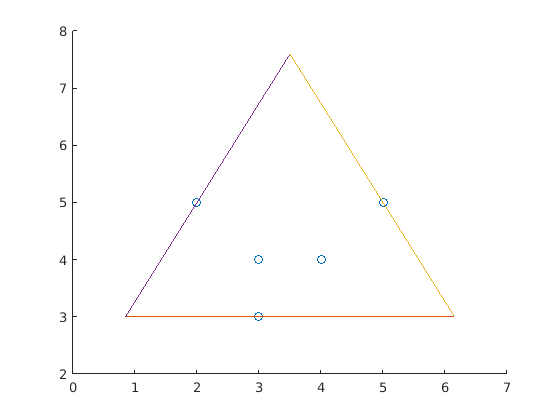
\includegraphics[width=0.75\linewidth]{results-1}
	\caption{Smallest equilateral triangle to enclose the sequence of points \{(3,3), (3,4), (4,4), (5,5), (2,5)\}.}
\end{figure}

\newpage

\section{Problem 2: Duality}

We are given the linear program:

\begin{align*}
&\max_\mathbf{x} \mathbf{c}^T \mathbf{x} \\
\text{subject to} & \hspace{0.1in} x_1 + x_2 + ... + x_n = 1\\
&x_i \ge 0, \forall i
\end{align*}

\subsection{What is the dual for this problem?}

First we rewrite the LP as its corresponding minimization problem,

\begin{align*}
&\min_\mathbf{x} -\mathbf{c}^T \mathbf{x} \\
\text{subject to} & \hspace{0.1in} x_1 + x_2 + ... + x_n = 1\\
&x_i \ge 0, \forall i
\end{align*}

The dual of this LP is a maximization problem.
The constraints of the primal become the costs in the dual; and the costs in the primal become part of the constraints in the dual.
The dual should have one unknown, as the primal has one constraint; and the dual should have \textit{n} constraints.
The last thing to consider when mapping this linear program to its dual is that equalities in the primal constraints correspond to free variables in the dual.
This means the unknown in the dual is free.
The dual is given formally by,

\begin{align*}
&\max_{u, v} u - v \\
\text{subject to} & \hspace{0.1in} u - v \le -c_1\\
& \hspace{0.1in} u - v \le -c_2\\
& \hspace{0.1in} \vdots \hspace{0.5in} \vdots\\
& \hspace{0.1in} u - v \le -c_n\\ 
&u, v \ge 0
\end{align*}

\subsection{Assume that $c_1$ is the largest coefficient of the cost vector, what is the solution of the dual?}

If $c_1 = \max(\mathbf{c})$ then $-c_1 \le -c_i$ for every $i$.
It is obvious then that any choice of $u$ and $v$ that satisfy $u - v \le -c_1$ will also satisfy the rest of the constraints.
The maximum $u - v$ is equal to $-c_1$.
The solution to the dual is any choice of $u$ and $v$ such that $u - v = -c_1$ and $u, v \ge 0$, say $u = 0$ and $v = c_1$.
The cost associated with this solution is $-c_1$.

\subsection{Using the solution of the dual, find the solution of the primal.}

Because an optimal solution exists for the dual, we know that an optimal solution exists for the primal, and that its cost is equal to $-c_1$ (in the case of the primal LP being in the form: $\min_\mathbf{x} -\mathbf{c}^T \mathbf{x}$). This is true if $x_1 = 1$ and $x_i = 0$ for every $i > 1$. The solution to the primal then is $\mathbf{x} = \begin{bmatrix}1 & 0 & 0 & \dots & 0\end{bmatrix}^T$.

\newpage

\section{Problem 3: Duality}

A newly published algorithm has reported that the following linear program has $\mathbf{x}_0 = \begin{bmatrix} 0 & 1 & 0 & 6 \end{bmatrix}^T$ as the optimal solution.

\begin{align*}
\text{max} & \hspace{0.1in} x_1 + x_2 + x_3 + 2x_4\\
\text{subject to} & \hspace{0.1in} x_1 + x_2 \le 2\\
& \hspace{0.1in} x_3 + x_4 \le 6\\
& \hspace{0.1in} x_i \ge 0, \forall i
\end{align*}

\subsection{What is the value of the slack variables in the primal?} \label{sec:slack_primal}

We can arrive at the values of the slack variables by rewriting the constraints as equalities with slack variables and plugging the solution into the constraints. Formally,

\begin{align*}
0 + 1 + s_1 = 2\\
0 + 6 + s_2 = 6
\end{align*}

\noindent where $s_1$ and $s_2$ are the slack variables. Some elementary algebra yields $s_1 = 1$ and $s_2 = 0$.

\subsection{What is the dual for this problem?}

The LP is of the form,

\begin{align*}
\max_\mathbf{x} & \hspace{0.1in} \mathbf{b}^T \mathbf{x}\\
\text{subject to} & \hspace{0.1in} \mathbf{A}^T \mathbf{x} \le \mathbf{c}^T\\
& \hspace{0.1in} x_i \ge 0, \forall i
\end{align*}

\noindent where, $\mathbf{b} = \begin{bmatrix}1 & 1 & 1 & 2\end{bmatrix}^T$, $\mathbf{A}^T = \left[\begin{smallmatrix}1 & 1 & 0 & 0\\0 & 0 & 1 & 1\end{smallmatrix}\right]$, and $\mathbf{c}^T = \begin{bmatrix} 2 & 6 \end{bmatrix}$.

Its dual is,

\begin{align*}
\min_{\boldsymbol{\lambda}} & \hspace{0.1in} \mathbf{c}^T \boldsymbol{\lambda}\\
\text{subject to} & \hspace{0.1in} \mathbf{A} \boldsymbol{\lambda} \ge \mathbf{b}\\
& \hspace{0.1in} \lambda_i \ge 0, \forall i
\end{align*}

or alternatively,

\begin{align*}
\text{min} & \hspace{0.1in} 2\lambda_1 + 6\lambda_2\\
\text{subject to} & \hspace{0.1in} \lambda_1 \ge 1\\
& \hspace{0.1in} \lambda_1 \ge 1\\
& \hspace{0.1in} \lambda_2 \ge 1\\
& \hspace{0.1in} \lambda_2 \ge 2\\
& \hspace{0.1in} \lambda_i \ge 0, \forall i
\end{align*}

\subsection{Solve the dual by inspection}

The solution of the dual is $\lambda_1 = 1$ and $\lambda_2 = 2$.

\subsection{Using complementary slackness, can you tell if the solution $\mathbf{x}_0$ is optimal?} \label{sec:compl_slack}

We can arrive at the values of the slack variables for the dual by the same process we used with the primal (see Section \ref{sec:slack_primal}). Formally,

\begin{align*}
1 - t_1 = 1\\
1 - t_2 = 1\\
2 - t_3 = 1\\
2 - t_4 = 2
\end{align*}

\noindent where $t_1$, $t_2$, $t_3$, and $t_4$ are the slack variables. Some elementary algebra yields $t_1 = 0$, $t_2 = 0$, $t_3 = 1$, and $t_4 = 0$.

A pair of primal and dual solutions $\mathbf{x}$ and $\boldsymbol{\lambda}$ are optimal if and only if $\mathbf{x}^T \mathbf{t} = 0$ and $\boldsymbol{\lambda}^T \mathbf{s} = 0$, where $\mathbf{s}$ and $\mathbf{t}$ are the slack variables for the primal and dual respectively.
For the given problem, $\mathbf{x}_0^T \mathbf{t} = 0$ and $\boldsymbol{\lambda}^T \mathbf{s} = 1$, hence $\mathbf{x}_0$ and $\boldsymbol{\lambda}$ are not optimal solutions.

\subsection{Using the solution of the dual, find the solution of the primal. Show all the steps.}

A pair of primal and dual solutions $\mathbf{x}$ and $\boldsymbol{\lambda}$ are optimal if and only if $\mathbf{c}^T \mathbf{x} = \boldsymbol{\lambda}^T \mathbf{b}$.
By inspection, the optimal solution of the dual LP is $\boldsymbol{\lambda} = \begin{bmatrix}1 & 2\end{bmatrix}$, which has a cost of 14.
Hence, the optimal solution for the primal satisfies the condition $\mathbf{c}^T \mathbf{x} = 14$.
We can use this to determine the optimal solution of the primal:

\begin{align} \label{eq:primal_const1}
x_1 + x_2 + x_3 + 2x_4 = 14\\\label{eq:primal_const2}
x_1 + x_2 \le 2\\\label{eq:primal_const3}
x_3 + x_4 \le 6\\
x_i \ge 0, \forall i
\end{align}

\noindent For any choice of $x_1$ and $x_2$ such that $x_1 + x_2 = 2$ and $x_1, x_2 \ge 0$ the first constraint, (\ref{eq:primal_const2}), is satisfied and the cost function is maximized.
Plugging $x_1$ and $x_2 $ into (\ref{eq:primal_const1}), the system of equations becomes

\begin{align*}
x_3 + 2x_4 = 12\\
x_3 + x_4 \le 6\\
x_i \ge 0, \forall i
\end{align*}

\noindent and can only be satisfied if $x_3 = 0$ and $x_4 = 6$. The three possible optimal solutions are $\mathbf{x}_1 = \begin{bmatrix}1 & 1 & 0 & 6\end{bmatrix}^T$, $\mathbf{x}_2 = \begin{bmatrix}2 & 0 & 0 & 6\end{bmatrix}^T$, and $\mathbf{x}_1 = \begin{bmatrix}0 & 2 & 0 & 6\end{bmatrix}^T$.
The fact that $\mathbf{x}_0$ is not among the optimal solutions agrees with the answer given in Section \ref{sec:compl_slack}. 
We also find that for $\mathbf{x}_1$, $\mathbf{x}_2$, and $\mathbf{x}_3$, the slack variables, $s_1$ and $s_2$ are equal to zero.
This gives us $\mathbf{x}_j^T \mathbf{t} = 0$ and $\boldsymbol{\lambda}^T \mathbf{s}_j = 0$ for $j = 1, 2, 3$, satisfying the complementary slackness criteria for optimal solutions.

\newpage

\section{Problem 4: Absolute Value Problem}

Convert the following problem into a linear program and solve using \texttt{linprog}.

\begin{align*}
\text{min} & \hspace{0.1in} x_1 + |x_2 - x_3|\\
\text{subject to} & \hspace{0.1in} |x_1 - 3| + |x_2 + 2| \le 7\\
& \hspace{0.1in} \sqrt{x_3 - x_1} \le 3\\
\end{align*}



\end{document}